% Created by tikzDevice version 0.8.1 on 2016-07-07 17:30:20
% !TEX encoding = UTF-8 Unicode
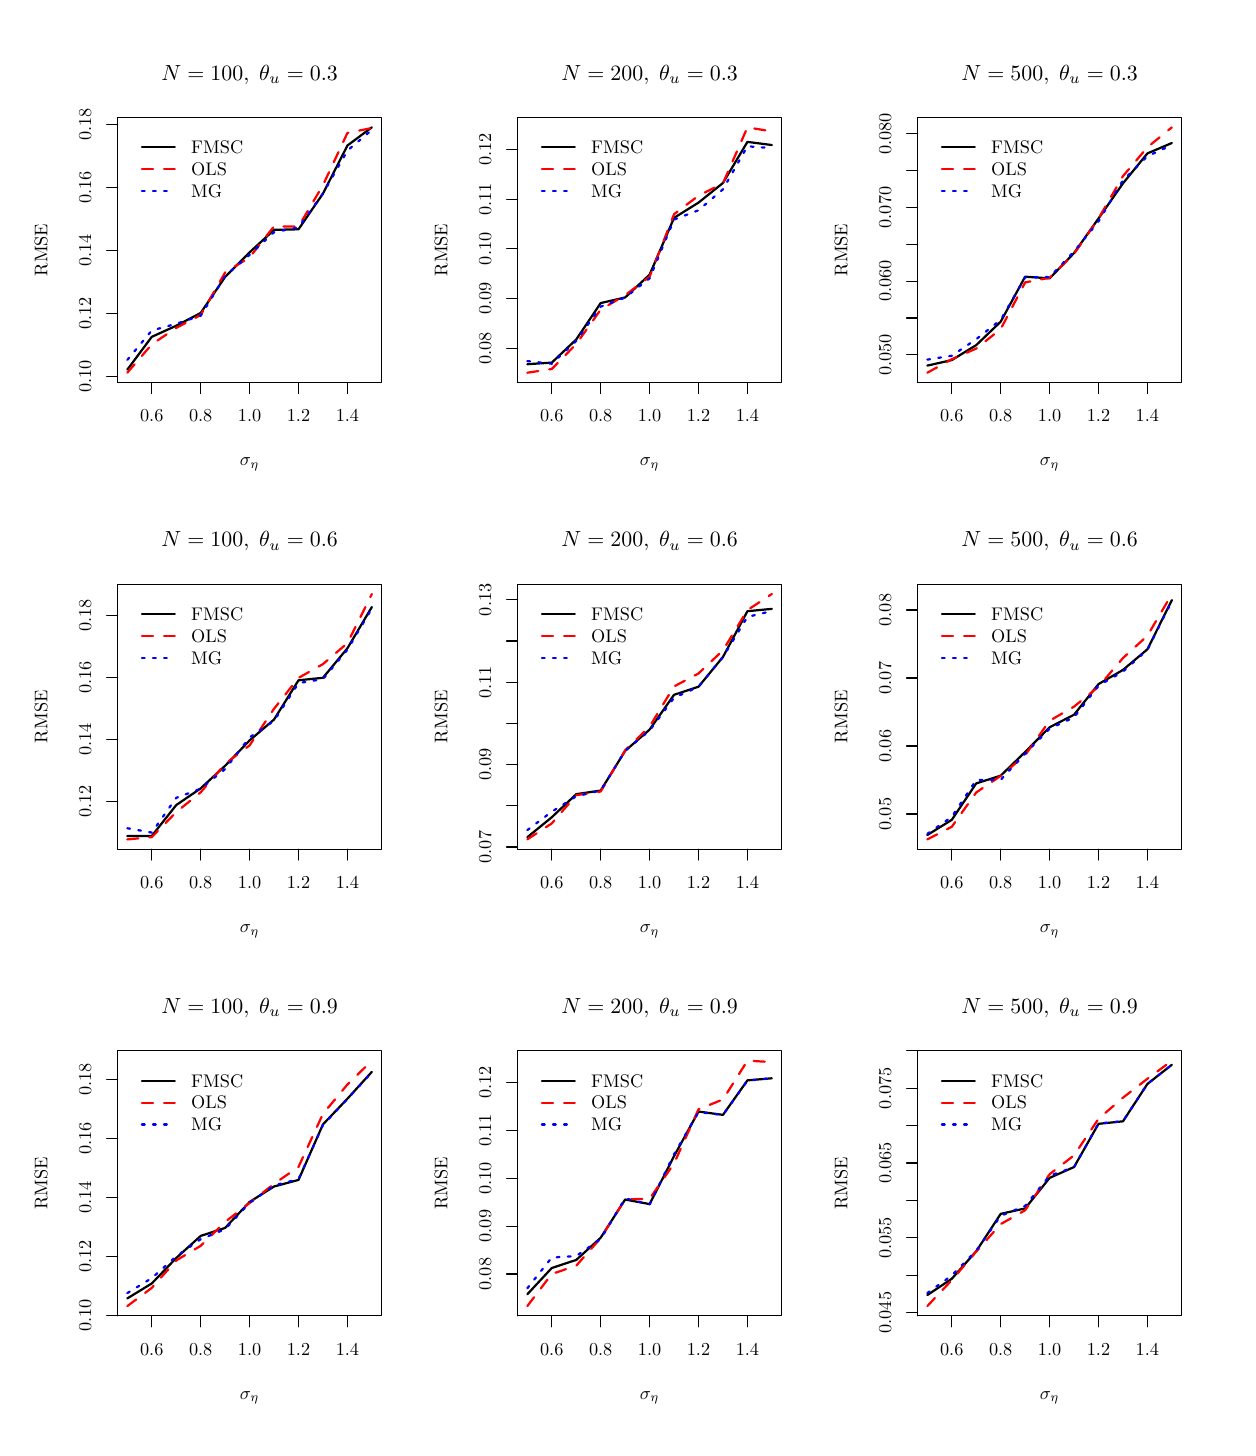
\begin{tikzpicture}[x=1pt,y=1pt]
\definecolor{fillColor}{RGB}{255,255,255}
\path[use as bounding box,fill=fillColor,fill opacity=0.00] (0,0) rectangle (433.62,505.89);
\begin{scope}
\path[clip] ( 32.47,377.65) rectangle (127.91,473.42);
\definecolor{drawColor}{RGB}{0,0,0}

\path[draw=drawColor,line width= 0.8pt,line join=round,line cap=round] ( 36.01,382.32) --
	( 44.84,394.16) --
	( 53.68,398.18) --
	( 62.52,402.80) --
	( 71.35,415.82) --
	( 80.19,424.69) --
	( 89.03,432.84) --
	( 97.86,433.02) --
	(106.70,445.93) --
	(115.54,463.30) --
	(124.37,469.87);
\end{scope}
\begin{scope}
\path[clip] (  0.00,  0.00) rectangle (433.62,505.89);
\definecolor{drawColor}{RGB}{0,0,0}

\path[draw=drawColor,line width= 0.4pt,line join=round,line cap=round] ( 44.84,377.65) -- (115.54,377.65);

\path[draw=drawColor,line width= 0.4pt,line join=round,line cap=round] ( 44.84,377.65) -- ( 44.84,373.69);

\path[draw=drawColor,line width= 0.4pt,line join=round,line cap=round] ( 62.52,377.65) -- ( 62.52,373.69);

\path[draw=drawColor,line width= 0.4pt,line join=round,line cap=round] ( 80.19,377.65) -- ( 80.19,373.69);

\path[draw=drawColor,line width= 0.4pt,line join=round,line cap=round] ( 97.86,377.65) -- ( 97.86,373.69);

\path[draw=drawColor,line width= 0.4pt,line join=round,line cap=round] (115.54,377.65) -- (115.54,373.69);

\node[text=drawColor,anchor=base,inner sep=0pt, outer sep=0pt, scale=  0.66] at ( 44.84,363.40) {0.6};

\node[text=drawColor,anchor=base,inner sep=0pt, outer sep=0pt, scale=  0.66] at ( 62.52,363.40) {0.8};

\node[text=drawColor,anchor=base,inner sep=0pt, outer sep=0pt, scale=  0.66] at ( 80.19,363.40) {1.0};

\node[text=drawColor,anchor=base,inner sep=0pt, outer sep=0pt, scale=  0.66] at ( 97.86,363.40) {1.2};

\node[text=drawColor,anchor=base,inner sep=0pt, outer sep=0pt, scale=  0.66] at (115.54,363.40) {1.4};

\path[draw=drawColor,line width= 0.4pt,line join=round,line cap=round] ( 32.47,379.95) -- ( 32.47,470.83);

\path[draw=drawColor,line width= 0.4pt,line join=round,line cap=round] ( 32.47,379.95) -- ( 28.51,379.95);

\path[draw=drawColor,line width= 0.4pt,line join=round,line cap=round] ( 32.47,402.67) -- ( 28.51,402.67);

\path[draw=drawColor,line width= 0.4pt,line join=round,line cap=round] ( 32.47,425.39) -- ( 28.51,425.39);

\path[draw=drawColor,line width= 0.4pt,line join=round,line cap=round] ( 32.47,448.11) -- ( 28.51,448.11);

\path[draw=drawColor,line width= 0.4pt,line join=round,line cap=round] ( 32.47,470.83) -- ( 28.51,470.83);

\node[text=drawColor,rotate= 90.00,anchor=base,inner sep=0pt, outer sep=0pt, scale=  0.66] at ( 22.97,379.95) {0.10};

\node[text=drawColor,rotate= 90.00,anchor=base,inner sep=0pt, outer sep=0pt, scale=  0.66] at ( 22.97,402.67) {0.12};

\node[text=drawColor,rotate= 90.00,anchor=base,inner sep=0pt, outer sep=0pt, scale=  0.66] at ( 22.97,425.39) {0.14};

\node[text=drawColor,rotate= 90.00,anchor=base,inner sep=0pt, outer sep=0pt, scale=  0.66] at ( 22.97,448.11) {0.16};

\node[text=drawColor,rotate= 90.00,anchor=base,inner sep=0pt, outer sep=0pt, scale=  0.66] at ( 22.97,470.83) {0.18};

\path[draw=drawColor,line width= 0.4pt,line join=round,line cap=round] ( 32.47,377.65) --
	(127.91,377.65) --
	(127.91,473.42) --
	( 32.47,473.42) --
	( 32.47,377.65);
\end{scope}
\begin{scope}
\path[clip] (  0.00,337.26) rectangle (144.54,505.89);
\definecolor{drawColor}{RGB}{0,0,0}

\node[text=drawColor,anchor=base,inner sep=0pt, outer sep=0pt, scale=  0.79] at ( 80.19,486.92) {\bfseries $N=100, \;\theta_u=0.3$};

\node[text=drawColor,anchor=base,inner sep=0pt, outer sep=0pt, scale=  0.66] at ( 80.19,347.56) {$\sigma_\eta$};

\node[text=drawColor,rotate= 90.00,anchor=base,inner sep=0pt, outer sep=0pt, scale=  0.66] at (  7.13,425.53) {RMSE};
\end{scope}
\begin{scope}
\path[clip] ( 32.47,377.65) rectangle (127.91,473.42);
\definecolor{drawColor}{RGB}{255,0,0}

\path[draw=drawColor,line width= 0.8pt,dash pattern=on 4pt off 4pt ,line join=round,line cap=round] ( 36.01,381.20) --
	( 44.84,391.46) --
	( 53.68,397.39) --
	( 62.52,402.04) --
	( 71.35,417.41) --
	( 80.19,422.90) --
	( 89.03,434.11) --
	( 97.86,433.98) --
	(106.70,448.98) --
	(115.54,467.83) --
	(124.37,469.64);
\definecolor{drawColor}{RGB}{0,0,255}

\path[draw=drawColor,line width= 0.8pt,dash pattern=on 1pt off 3pt ,line join=round,line cap=round] ( 36.01,385.83) --
	( 44.84,396.46) --
	( 53.68,398.88) --
	( 62.52,401.78) --
	( 71.35,416.13) --
	( 80.19,423.80) --
	( 89.03,431.98) --
	( 97.86,433.69) --
	(106.70,445.96) --
	(115.54,461.47) --
	(124.37,468.94);
\definecolor{drawColor}{RGB}{0,0,0}

\path[draw=drawColor,line width= 0.8pt,line join=round,line cap=round] ( 41.28,462.63) -- ( 53.16,462.63);
\definecolor{drawColor}{RGB}{255,0,0}

\path[draw=drawColor,line width= 0.8pt,dash pattern=on 4pt off 4pt ,line join=round,line cap=round] ( 41.28,454.71) -- ( 53.16,454.71);
\definecolor{drawColor}{RGB}{0,0,255}

\path[draw=drawColor,line width= 0.8pt,dash pattern=on 1pt off 3pt ,line join=round,line cap=round] ( 41.28,446.79) -- ( 53.16,446.79);
\definecolor{drawColor}{RGB}{0,0,0}

\node[text=drawColor,anchor=base west,inner sep=0pt, outer sep=0pt, scale=  0.66] at ( 59.10,460.35) {FMSC};

\node[text=drawColor,anchor=base west,inner sep=0pt, outer sep=0pt, scale=  0.66] at ( 59.10,452.43) {OLS};

\node[text=drawColor,anchor=base west,inner sep=0pt, outer sep=0pt, scale=  0.66] at ( 59.10,444.51) {MG};
\end{scope}
\begin{scope}
\path[clip] (177.01,377.65) rectangle (272.45,473.42);
\definecolor{drawColor}{RGB}{0,0,0}

\path[draw=drawColor,line width= 0.8pt,line join=round,line cap=round] (180.55,384.28) --
	(189.38,384.85) --
	(198.22,393.22) --
	(207.06,406.37) --
	(215.89,408.40) --
	(224.73,416.63) --
	(233.57,437.17) --
	(242.40,442.66) --
	(251.24,449.77) --
	(260.08,464.61) --
	(268.91,463.48);
\end{scope}
\begin{scope}
\path[clip] (  0.00,  0.00) rectangle (433.62,505.89);
\definecolor{drawColor}{RGB}{0,0,0}

\path[draw=drawColor,line width= 0.4pt,line join=round,line cap=round] (189.38,377.65) -- (260.08,377.65);

\path[draw=drawColor,line width= 0.4pt,line join=round,line cap=round] (189.38,377.65) -- (189.38,373.69);

\path[draw=drawColor,line width= 0.4pt,line join=round,line cap=round] (207.06,377.65) -- (207.06,373.69);

\path[draw=drawColor,line width= 0.4pt,line join=round,line cap=round] (224.73,377.65) -- (224.73,373.69);

\path[draw=drawColor,line width= 0.4pt,line join=round,line cap=round] (242.40,377.65) -- (242.40,373.69);

\path[draw=drawColor,line width= 0.4pt,line join=round,line cap=round] (260.08,377.65) -- (260.08,373.69);

\node[text=drawColor,anchor=base,inner sep=0pt, outer sep=0pt, scale=  0.66] at (189.38,363.40) {0.6};

\node[text=drawColor,anchor=base,inner sep=0pt, outer sep=0pt, scale=  0.66] at (207.06,363.40) {0.8};

\node[text=drawColor,anchor=base,inner sep=0pt, outer sep=0pt, scale=  0.66] at (224.73,363.40) {1.0};

\node[text=drawColor,anchor=base,inner sep=0pt, outer sep=0pt, scale=  0.66] at (242.40,363.40) {1.2};

\node[text=drawColor,anchor=base,inner sep=0pt, outer sep=0pt, scale=  0.66] at (260.08,363.40) {1.4};

\path[draw=drawColor,line width= 0.4pt,line join=round,line cap=round] (177.01,390.07) -- (177.01,461.88);

\path[draw=drawColor,line width= 0.4pt,line join=round,line cap=round] (177.01,390.07) -- (173.05,390.07);

\path[draw=drawColor,line width= 0.4pt,line join=round,line cap=round] (177.01,408.02) -- (173.05,408.02);

\path[draw=drawColor,line width= 0.4pt,line join=round,line cap=round] (177.01,425.97) -- (173.05,425.97);

\path[draw=drawColor,line width= 0.4pt,line join=round,line cap=round] (177.01,443.92) -- (173.05,443.92);

\path[draw=drawColor,line width= 0.4pt,line join=round,line cap=round] (177.01,461.88) -- (173.05,461.88);

\node[text=drawColor,rotate= 90.00,anchor=base,inner sep=0pt, outer sep=0pt, scale=  0.66] at (167.51,390.07) {0.08};

\node[text=drawColor,rotate= 90.00,anchor=base,inner sep=0pt, outer sep=0pt, scale=  0.66] at (167.51,408.02) {0.09};

\node[text=drawColor,rotate= 90.00,anchor=base,inner sep=0pt, outer sep=0pt, scale=  0.66] at (167.51,425.97) {0.10};

\node[text=drawColor,rotate= 90.00,anchor=base,inner sep=0pt, outer sep=0pt, scale=  0.66] at (167.51,443.92) {0.11};

\node[text=drawColor,rotate= 90.00,anchor=base,inner sep=0pt, outer sep=0pt, scale=  0.66] at (167.51,461.88) {0.12};

\path[draw=drawColor,line width= 0.4pt,line join=round,line cap=round] (177.01,377.65) --
	(272.45,377.65) --
	(272.45,473.42) --
	(177.01,473.42) --
	(177.01,377.65);
\end{scope}
\begin{scope}
\path[clip] (144.54,337.26) rectangle (289.08,505.89);
\definecolor{drawColor}{RGB}{0,0,0}

\node[text=drawColor,anchor=base,inner sep=0pt, outer sep=0pt, scale=  0.79] at (224.73,486.92) {\bfseries $N=200, \;\theta_u=0.3$};

\node[text=drawColor,anchor=base,inner sep=0pt, outer sep=0pt, scale=  0.66] at (224.73,347.56) {$\sigma_\eta$};

\node[text=drawColor,rotate= 90.00,anchor=base,inner sep=0pt, outer sep=0pt, scale=  0.66] at (151.67,425.53) {RMSE};
\end{scope}
\begin{scope}
\path[clip] (177.01,377.65) rectangle (272.45,473.42);
\definecolor{drawColor}{RGB}{255,0,0}

\path[draw=drawColor,line width= 0.8pt,dash pattern=on 4pt off 4pt ,line join=round,line cap=round] (180.55,381.20) --
	(189.38,382.54) --
	(198.22,391.56) --
	(207.06,404.00) --
	(215.89,409.22) --
	(224.73,415.90) --
	(233.57,438.48) --
	(242.40,445.16) --
	(251.24,449.64) --
	(260.08,469.87) --
	(268.91,468.40);
\definecolor{drawColor}{RGB}{0,0,255}

\path[draw=drawColor,line width= 0.8pt,dash pattern=on 1pt off 3pt ,line join=round,line cap=round] (180.55,385.40) --
	(189.38,384.46) --
	(198.22,392.68) --
	(207.06,405.08) --
	(215.89,408.37) --
	(224.73,415.30) --
	(233.57,436.54) --
	(242.40,439.90) --
	(251.24,447.48) --
	(260.08,463.02) --
	(268.91,462.36);
\definecolor{drawColor}{RGB}{0,0,0}

\path[draw=drawColor,line width= 0.8pt,line join=round,line cap=round] (185.82,462.63) -- (197.70,462.63);
\definecolor{drawColor}{RGB}{255,0,0}

\path[draw=drawColor,line width= 0.8pt,dash pattern=on 4pt off 4pt ,line join=round,line cap=round] (185.82,454.71) -- (197.70,454.71);
\definecolor{drawColor}{RGB}{0,0,255}

\path[draw=drawColor,line width= 0.8pt,dash pattern=on 1pt off 3pt ,line join=round,line cap=round] (185.82,446.79) -- (197.70,446.79);
\definecolor{drawColor}{RGB}{0,0,0}

\node[text=drawColor,anchor=base west,inner sep=0pt, outer sep=0pt, scale=  0.66] at (203.64,460.35) {FMSC};

\node[text=drawColor,anchor=base west,inner sep=0pt, outer sep=0pt, scale=  0.66] at (203.64,452.43) {OLS};

\node[text=drawColor,anchor=base west,inner sep=0pt, outer sep=0pt, scale=  0.66] at (203.64,444.51) {MG};
\end{scope}
\begin{scope}
\path[clip] (321.55,377.65) rectangle (416.99,473.42);
\definecolor{drawColor}{RGB}{0,0,0}

\path[draw=drawColor,line width= 0.8pt,line join=round,line cap=round] (325.09,383.77) --
	(333.92,385.76) --
	(342.76,391.18) --
	(351.60,399.65) --
	(360.43,415.90) --
	(369.27,415.30) --
	(378.11,424.45) --
	(386.94,436.94) --
	(395.78,449.63) --
	(404.62,460.45) --
	(413.45,464.21);
\end{scope}
\begin{scope}
\path[clip] (  0.00,  0.00) rectangle (433.62,505.89);
\definecolor{drawColor}{RGB}{0,0,0}

\path[draw=drawColor,line width= 0.4pt,line join=round,line cap=round] (333.92,377.65) -- (404.62,377.65);

\path[draw=drawColor,line width= 0.4pt,line join=round,line cap=round] (333.92,377.65) -- (333.92,373.69);

\path[draw=drawColor,line width= 0.4pt,line join=round,line cap=round] (351.60,377.65) -- (351.60,373.69);

\path[draw=drawColor,line width= 0.4pt,line join=round,line cap=round] (369.27,377.65) -- (369.27,373.69);

\path[draw=drawColor,line width= 0.4pt,line join=round,line cap=round] (386.94,377.65) -- (386.94,373.69);

\path[draw=drawColor,line width= 0.4pt,line join=round,line cap=round] (404.62,377.65) -- (404.62,373.69);

\node[text=drawColor,anchor=base,inner sep=0pt, outer sep=0pt, scale=  0.66] at (333.92,363.40) {0.6};

\node[text=drawColor,anchor=base,inner sep=0pt, outer sep=0pt, scale=  0.66] at (351.60,363.40) {0.8};

\node[text=drawColor,anchor=base,inner sep=0pt, outer sep=0pt, scale=  0.66] at (369.27,363.40) {1.0};

\node[text=drawColor,anchor=base,inner sep=0pt, outer sep=0pt, scale=  0.66] at (386.94,363.40) {1.2};

\node[text=drawColor,anchor=base,inner sep=0pt, outer sep=0pt, scale=  0.66] at (404.62,363.40) {1.4};

\path[draw=drawColor,line width= 0.4pt,line join=round,line cap=round] (321.55,387.68) -- (321.55,467.50);

\path[draw=drawColor,line width= 0.4pt,line join=round,line cap=round] (321.55,387.68) -- (317.59,387.68);

\path[draw=drawColor,line width= 0.4pt,line join=round,line cap=round] (321.55,400.99) -- (317.59,400.99);

\path[draw=drawColor,line width= 0.4pt,line join=round,line cap=round] (321.55,414.29) -- (317.59,414.29);

\path[draw=drawColor,line width= 0.4pt,line join=round,line cap=round] (321.55,427.59) -- (317.59,427.59);

\path[draw=drawColor,line width= 0.4pt,line join=round,line cap=round] (321.55,440.90) -- (317.59,440.90);

\path[draw=drawColor,line width= 0.4pt,line join=round,line cap=round] (321.55,454.20) -- (317.59,454.20);

\path[draw=drawColor,line width= 0.4pt,line join=round,line cap=round] (321.55,467.50) -- (317.59,467.50);

\node[text=drawColor,rotate= 90.00,anchor=base,inner sep=0pt, outer sep=0pt, scale=  0.66] at (312.05,387.68) {0.050};

\node[text=drawColor,rotate= 90.00,anchor=base,inner sep=0pt, outer sep=0pt, scale=  0.66] at (312.05,414.29) {0.060};

\node[text=drawColor,rotate= 90.00,anchor=base,inner sep=0pt, outer sep=0pt, scale=  0.66] at (312.05,440.90) {0.070};

\node[text=drawColor,rotate= 90.00,anchor=base,inner sep=0pt, outer sep=0pt, scale=  0.66] at (312.05,467.50) {0.080};

\path[draw=drawColor,line width= 0.4pt,line join=round,line cap=round] (321.55,377.65) --
	(416.99,377.65) --
	(416.99,473.42) --
	(321.55,473.42) --
	(321.55,377.65);
\end{scope}
\begin{scope}
\path[clip] (289.08,337.26) rectangle (433.62,505.89);
\definecolor{drawColor}{RGB}{0,0,0}

\node[text=drawColor,anchor=base,inner sep=0pt, outer sep=0pt, scale=  0.79] at (369.27,486.92) {\bfseries $N=500, \;\theta_u=0.3$};

\node[text=drawColor,anchor=base,inner sep=0pt, outer sep=0pt, scale=  0.66] at (369.27,347.56) {$\sigma_\eta$};

\node[text=drawColor,rotate= 90.00,anchor=base,inner sep=0pt, outer sep=0pt, scale=  0.66] at (296.21,425.53) {RMSE};
\end{scope}
\begin{scope}
\path[clip] (321.55,377.65) rectangle (416.99,473.42);
\definecolor{drawColor}{RGB}{255,0,0}

\path[draw=drawColor,line width= 0.8pt,dash pattern=on 4pt off 4pt ,line join=round,line cap=round] (325.09,381.20) --
	(333.92,386.09) --
	(342.76,389.94) --
	(351.60,396.98) --
	(360.43,413.84) --
	(369.27,415.51) --
	(378.11,424.15) --
	(386.94,436.90) --
	(395.78,452.24) --
	(404.62,462.68) --
	(413.45,469.87);
\definecolor{drawColor}{RGB}{0,0,255}

\path[draw=drawColor,line width= 0.8pt,dash pattern=on 1pt off 3pt ,line join=round,line cap=round] (325.09,385.94) --
	(333.92,387.34) --
	(342.76,393.32) --
	(351.60,400.29) --
	(360.43,415.67) --
	(369.27,415.77) --
	(378.11,425.00) --
	(386.94,435.88) --
	(395.78,450.73) --
	(404.62,459.45) --
	(413.45,463.47);
\definecolor{drawColor}{RGB}{0,0,0}

\path[draw=drawColor,line width= 0.8pt,line join=round,line cap=round] (330.36,462.63) -- (342.24,462.63);
\definecolor{drawColor}{RGB}{255,0,0}

\path[draw=drawColor,line width= 0.8pt,dash pattern=on 4pt off 4pt ,line join=round,line cap=round] (330.36,454.71) -- (342.24,454.71);
\definecolor{drawColor}{RGB}{0,0,255}

\path[draw=drawColor,line width= 0.8pt,dash pattern=on 1pt off 3pt ,line join=round,line cap=round] (330.36,446.79) -- (342.24,446.79);
\definecolor{drawColor}{RGB}{0,0,0}

\node[text=drawColor,anchor=base west,inner sep=0pt, outer sep=0pt, scale=  0.66] at (348.18,460.35) {FMSC};

\node[text=drawColor,anchor=base west,inner sep=0pt, outer sep=0pt, scale=  0.66] at (348.18,452.43) {OLS};

\node[text=drawColor,anchor=base west,inner sep=0pt, outer sep=0pt, scale=  0.66] at (348.18,444.51) {MG};
\end{scope}
\begin{scope}
\path[clip] ( 32.47,209.02) rectangle (127.91,304.79);
\definecolor{drawColor}{RGB}{0,0,0}

\path[draw=drawColor,line width= 0.8pt,line join=round,line cap=round] ( 36.01,213.79) --
	( 44.84,213.81) --
	( 53.68,224.97) --
	( 62.52,231.01) --
	( 71.35,239.18) --
	( 80.19,248.33) --
	( 89.03,255.90) --
	( 97.86,270.06) --
	(106.70,270.97) --
	(115.54,281.64) --
	(124.37,296.55);
\end{scope}
\begin{scope}
\path[clip] (  0.00,  0.00) rectangle (433.62,505.89);
\definecolor{drawColor}{RGB}{0,0,0}

\path[draw=drawColor,line width= 0.4pt,line join=round,line cap=round] ( 44.84,209.02) -- (115.54,209.02);

\path[draw=drawColor,line width= 0.4pt,line join=round,line cap=round] ( 44.84,209.02) -- ( 44.84,205.06);

\path[draw=drawColor,line width= 0.4pt,line join=round,line cap=round] ( 62.52,209.02) -- ( 62.52,205.06);

\path[draw=drawColor,line width= 0.4pt,line join=round,line cap=round] ( 80.19,209.02) -- ( 80.19,205.06);

\path[draw=drawColor,line width= 0.4pt,line join=round,line cap=round] ( 97.86,209.02) -- ( 97.86,205.06);

\path[draw=drawColor,line width= 0.4pt,line join=round,line cap=round] (115.54,209.02) -- (115.54,205.06);

\node[text=drawColor,anchor=base,inner sep=0pt, outer sep=0pt, scale=  0.66] at ( 44.84,194.77) {0.6};

\node[text=drawColor,anchor=base,inner sep=0pt, outer sep=0pt, scale=  0.66] at ( 62.52,194.77) {0.8};

\node[text=drawColor,anchor=base,inner sep=0pt, outer sep=0pt, scale=  0.66] at ( 80.19,194.77) {1.0};

\node[text=drawColor,anchor=base,inner sep=0pt, outer sep=0pt, scale=  0.66] at ( 97.86,194.77) {1.2};

\node[text=drawColor,anchor=base,inner sep=0pt, outer sep=0pt, scale=  0.66] at (115.54,194.77) {1.4};

\path[draw=drawColor,line width= 0.4pt,line join=round,line cap=round] ( 32.47,226.39) -- ( 32.47,293.50);

\path[draw=drawColor,line width= 0.4pt,line join=round,line cap=round] ( 32.47,226.39) -- ( 28.51,226.39);

\path[draw=drawColor,line width= 0.4pt,line join=round,line cap=round] ( 32.47,248.76) -- ( 28.51,248.76);

\path[draw=drawColor,line width= 0.4pt,line join=round,line cap=round] ( 32.47,271.13) -- ( 28.51,271.13);

\path[draw=drawColor,line width= 0.4pt,line join=round,line cap=round] ( 32.47,293.50) -- ( 28.51,293.50);

\node[text=drawColor,rotate= 90.00,anchor=base,inner sep=0pt, outer sep=0pt, scale=  0.66] at ( 22.97,226.39) {0.12};

\node[text=drawColor,rotate= 90.00,anchor=base,inner sep=0pt, outer sep=0pt, scale=  0.66] at ( 22.97,248.76) {0.14};

\node[text=drawColor,rotate= 90.00,anchor=base,inner sep=0pt, outer sep=0pt, scale=  0.66] at ( 22.97,271.13) {0.16};

\node[text=drawColor,rotate= 90.00,anchor=base,inner sep=0pt, outer sep=0pt, scale=  0.66] at ( 22.97,293.50) {0.18};

\path[draw=drawColor,line width= 0.4pt,line join=round,line cap=round] ( 32.47,209.02) --
	(127.91,209.02) --
	(127.91,304.79) --
	( 32.47,304.79) --
	( 32.47,209.02);
\end{scope}
\begin{scope}
\path[clip] (  0.00,168.63) rectangle (144.54,337.26);
\definecolor{drawColor}{RGB}{0,0,0}

\node[text=drawColor,anchor=base,inner sep=0pt, outer sep=0pt, scale=  0.79] at ( 80.19,318.29) {\bfseries $N=100, \;\theta_u=0.6$};

\node[text=drawColor,anchor=base,inner sep=0pt, outer sep=0pt, scale=  0.66] at ( 80.19,178.93) {$\sigma_\eta$};

\node[text=drawColor,rotate= 90.00,anchor=base,inner sep=0pt, outer sep=0pt, scale=  0.66] at (  7.13,256.90) {RMSE};
\end{scope}
\begin{scope}
\path[clip] ( 32.47,209.02) rectangle (127.91,304.79);
\definecolor{drawColor}{RGB}{255,0,0}

\path[draw=drawColor,line width= 0.8pt,dash pattern=on 4pt off 4pt ,line join=round,line cap=round] ( 36.01,212.57) --
	( 44.84,213.39) --
	( 53.68,222.43) --
	( 62.52,229.59) --
	( 71.35,239.85) --
	( 80.19,246.54) --
	( 89.03,259.78) --
	( 97.86,270.92) --
	(106.70,275.91) --
	(115.54,283.50) --
	(124.37,301.24);
\definecolor{drawColor}{RGB}{0,0,255}

\path[draw=drawColor,line width= 0.8pt,dash pattern=on 1pt off 3pt ,line join=round,line cap=round] ( 36.01,216.61) --
	( 44.84,215.03) --
	( 53.68,227.58) --
	( 62.52,230.89) --
	( 71.35,237.98) --
	( 80.19,249.43) --
	( 89.03,255.41) --
	( 97.86,269.06) --
	(106.70,270.47) --
	(115.54,281.13) --
	(124.37,296.02);
\definecolor{drawColor}{RGB}{0,0,0}

\path[draw=drawColor,line width= 0.8pt,line join=round,line cap=round] ( 41.28,294.00) -- ( 53.16,294.00);
\definecolor{drawColor}{RGB}{255,0,0}

\path[draw=drawColor,line width= 0.8pt,dash pattern=on 4pt off 4pt ,line join=round,line cap=round] ( 41.28,286.08) -- ( 53.16,286.08);
\definecolor{drawColor}{RGB}{0,0,255}

\path[draw=drawColor,line width= 0.8pt,dash pattern=on 1pt off 3pt ,line join=round,line cap=round] ( 41.28,278.16) -- ( 53.16,278.16);
\definecolor{drawColor}{RGB}{0,0,0}

\node[text=drawColor,anchor=base west,inner sep=0pt, outer sep=0pt, scale=  0.66] at ( 59.10,291.72) {FMSC};

\node[text=drawColor,anchor=base west,inner sep=0pt, outer sep=0pt, scale=  0.66] at ( 59.10,283.80) {OLS};

\node[text=drawColor,anchor=base west,inner sep=0pt, outer sep=0pt, scale=  0.66] at ( 59.10,275.88) {MG};
\end{scope}
\begin{scope}
\path[clip] (177.01,209.02) rectangle (272.45,304.79);
\definecolor{drawColor}{RGB}{0,0,0}

\path[draw=drawColor,line width= 0.8pt,line join=round,line cap=round] (180.55,213.36) --
	(189.38,220.57) --
	(198.22,228.92) --
	(207.06,230.23) --
	(215.89,244.56) --
	(224.73,252.25) --
	(233.57,264.82) --
	(242.40,267.73) --
	(251.24,278.49) --
	(260.08,295.03) --
	(268.91,295.87);
\end{scope}
\begin{scope}
\path[clip] (  0.00,  0.00) rectangle (433.62,505.89);
\definecolor{drawColor}{RGB}{0,0,0}

\path[draw=drawColor,line width= 0.4pt,line join=round,line cap=round] (189.38,209.02) -- (260.08,209.02);

\path[draw=drawColor,line width= 0.4pt,line join=round,line cap=round] (189.38,209.02) -- (189.38,205.06);

\path[draw=drawColor,line width= 0.4pt,line join=round,line cap=round] (207.06,209.02) -- (207.06,205.06);

\path[draw=drawColor,line width= 0.4pt,line join=round,line cap=round] (224.73,209.02) -- (224.73,205.06);

\path[draw=drawColor,line width= 0.4pt,line join=round,line cap=round] (242.40,209.02) -- (242.40,205.06);

\path[draw=drawColor,line width= 0.4pt,line join=round,line cap=round] (260.08,209.02) -- (260.08,205.06);

\node[text=drawColor,anchor=base,inner sep=0pt, outer sep=0pt, scale=  0.66] at (189.38,194.77) {0.6};

\node[text=drawColor,anchor=base,inner sep=0pt, outer sep=0pt, scale=  0.66] at (207.06,194.77) {0.8};

\node[text=drawColor,anchor=base,inner sep=0pt, outer sep=0pt, scale=  0.66] at (224.73,194.77) {1.0};

\node[text=drawColor,anchor=base,inner sep=0pt, outer sep=0pt, scale=  0.66] at (242.40,194.77) {1.2};

\node[text=drawColor,anchor=base,inner sep=0pt, outer sep=0pt, scale=  0.66] at (260.08,194.77) {1.4};

\path[draw=drawColor,line width= 0.4pt,line join=round,line cap=round] (177.01,209.82) -- (177.01,299.13);

\path[draw=drawColor,line width= 0.4pt,line join=round,line cap=round] (177.01,209.82) -- (173.05,209.82);

\path[draw=drawColor,line width= 0.4pt,line join=round,line cap=round] (177.01,224.70) -- (173.05,224.70);

\path[draw=drawColor,line width= 0.4pt,line join=round,line cap=round] (177.01,239.59) -- (173.05,239.59);

\path[draw=drawColor,line width= 0.4pt,line join=round,line cap=round] (177.01,254.48) -- (173.05,254.48);

\path[draw=drawColor,line width= 0.4pt,line join=round,line cap=round] (177.01,269.36) -- (173.05,269.36);

\path[draw=drawColor,line width= 0.4pt,line join=round,line cap=round] (177.01,284.25) -- (173.05,284.25);

\path[draw=drawColor,line width= 0.4pt,line join=round,line cap=round] (177.01,299.13) -- (173.05,299.13);

\node[text=drawColor,rotate= 90.00,anchor=base,inner sep=0pt, outer sep=0pt, scale=  0.66] at (167.51,209.82) {0.07};

\node[text=drawColor,rotate= 90.00,anchor=base,inner sep=0pt, outer sep=0pt, scale=  0.66] at (167.51,239.59) {0.09};

\node[text=drawColor,rotate= 90.00,anchor=base,inner sep=0pt, outer sep=0pt, scale=  0.66] at (167.51,269.36) {0.11};

\node[text=drawColor,rotate= 90.00,anchor=base,inner sep=0pt, outer sep=0pt, scale=  0.66] at (167.51,299.13) {0.13};

\path[draw=drawColor,line width= 0.4pt,line join=round,line cap=round] (177.01,209.02) --
	(272.45,209.02) --
	(272.45,304.79) --
	(177.01,304.79) --
	(177.01,209.02);
\end{scope}
\begin{scope}
\path[clip] (144.54,168.63) rectangle (289.08,337.26);
\definecolor{drawColor}{RGB}{0,0,0}

\node[text=drawColor,anchor=base,inner sep=0pt, outer sep=0pt, scale=  0.79] at (224.73,318.29) {\bfseries $N=200, \;\theta_u=0.6$};

\node[text=drawColor,anchor=base,inner sep=0pt, outer sep=0pt, scale=  0.66] at (224.73,178.93) {$\sigma_\eta$};

\node[text=drawColor,rotate= 90.00,anchor=base,inner sep=0pt, outer sep=0pt, scale=  0.66] at (151.67,256.90) {RMSE};
\end{scope}
\begin{scope}
\path[clip] (177.01,209.02) rectangle (272.45,304.79);
\definecolor{drawColor}{RGB}{255,0,0}

\path[draw=drawColor,line width= 0.8pt,dash pattern=on 4pt off 4pt ,line join=round,line cap=round] (180.55,212.57) --
	(189.38,218.34) --
	(198.22,228.54) --
	(207.06,229.87) --
	(215.89,244.75) --
	(224.73,253.33) --
	(233.57,267.85) --
	(242.40,272.53) --
	(251.24,280.89) --
	(260.08,295.43) --
	(268.91,301.24);
\definecolor{drawColor}{RGB}{0,0,255}

\path[draw=drawColor,line width= 0.8pt,dash pattern=on 1pt off 3pt ,line join=round,line cap=round] (180.55,215.94) --
	(189.38,222.58) --
	(198.22,228.14) --
	(207.06,230.25) --
	(215.89,244.58) --
	(224.73,251.91) --
	(233.57,263.74) --
	(242.40,267.71) --
	(251.24,278.47) --
	(260.08,292.98) --
	(268.91,295.08);
\definecolor{drawColor}{RGB}{0,0,0}

\path[draw=drawColor,line width= 0.8pt,line join=round,line cap=round] (185.82,294.00) -- (197.70,294.00);
\definecolor{drawColor}{RGB}{255,0,0}

\path[draw=drawColor,line width= 0.8pt,dash pattern=on 4pt off 4pt ,line join=round,line cap=round] (185.82,286.08) -- (197.70,286.08);
\definecolor{drawColor}{RGB}{0,0,255}

\path[draw=drawColor,line width= 0.8pt,dash pattern=on 1pt off 3pt ,line join=round,line cap=round] (185.82,278.16) -- (197.70,278.16);
\definecolor{drawColor}{RGB}{0,0,0}

\node[text=drawColor,anchor=base west,inner sep=0pt, outer sep=0pt, scale=  0.66] at (203.64,291.72) {FMSC};

\node[text=drawColor,anchor=base west,inner sep=0pt, outer sep=0pt, scale=  0.66] at (203.64,283.80) {OLS};

\node[text=drawColor,anchor=base west,inner sep=0pt, outer sep=0pt, scale=  0.66] at (203.64,275.88) {MG};
\end{scope}
\begin{scope}
\path[clip] (321.55,209.02) rectangle (416.99,304.79);
\definecolor{drawColor}{RGB}{0,0,0}

\path[draw=drawColor,line width= 0.8pt,line join=round,line cap=round] (325.09,214.15) --
	(333.92,219.64) --
	(342.76,232.81) --
	(351.60,235.60) --
	(360.43,244.16) --
	(369.27,253.09) --
	(378.11,257.63) --
	(386.94,268.69) --
	(395.78,273.81) --
	(404.62,281.27) --
	(413.45,299.05);
\end{scope}
\begin{scope}
\path[clip] (  0.00,  0.00) rectangle (433.62,505.89);
\definecolor{drawColor}{RGB}{0,0,0}

\path[draw=drawColor,line width= 0.4pt,line join=round,line cap=round] (333.92,209.02) -- (404.62,209.02);

\path[draw=drawColor,line width= 0.4pt,line join=round,line cap=round] (333.92,209.02) -- (333.92,205.06);

\path[draw=drawColor,line width= 0.4pt,line join=round,line cap=round] (351.60,209.02) -- (351.60,205.06);

\path[draw=drawColor,line width= 0.4pt,line join=round,line cap=round] (369.27,209.02) -- (369.27,205.06);

\path[draw=drawColor,line width= 0.4pt,line join=round,line cap=round] (386.94,209.02) -- (386.94,205.06);

\path[draw=drawColor,line width= 0.4pt,line join=round,line cap=round] (404.62,209.02) -- (404.62,205.06);

\node[text=drawColor,anchor=base,inner sep=0pt, outer sep=0pt, scale=  0.66] at (333.92,194.77) {0.6};

\node[text=drawColor,anchor=base,inner sep=0pt, outer sep=0pt, scale=  0.66] at (351.60,194.77) {0.8};

\node[text=drawColor,anchor=base,inner sep=0pt, outer sep=0pt, scale=  0.66] at (369.27,194.77) {1.0};

\node[text=drawColor,anchor=base,inner sep=0pt, outer sep=0pt, scale=  0.66] at (386.94,194.77) {1.2};

\node[text=drawColor,anchor=base,inner sep=0pt, outer sep=0pt, scale=  0.66] at (404.62,194.77) {1.4};

\path[draw=drawColor,line width= 0.4pt,line join=round,line cap=round] (321.55,221.75) -- (321.55,295.45);

\path[draw=drawColor,line width= 0.4pt,line join=round,line cap=round] (321.55,221.75) -- (317.59,221.75);

\path[draw=drawColor,line width= 0.4pt,line join=round,line cap=round] (321.55,246.31) -- (317.59,246.31);

\path[draw=drawColor,line width= 0.4pt,line join=round,line cap=round] (321.55,270.88) -- (317.59,270.88);

\path[draw=drawColor,line width= 0.4pt,line join=round,line cap=round] (321.55,295.45) -- (317.59,295.45);

\node[text=drawColor,rotate= 90.00,anchor=base,inner sep=0pt, outer sep=0pt, scale=  0.66] at (312.05,221.75) {0.05};

\node[text=drawColor,rotate= 90.00,anchor=base,inner sep=0pt, outer sep=0pt, scale=  0.66] at (312.05,246.31) {0.06};

\node[text=drawColor,rotate= 90.00,anchor=base,inner sep=0pt, outer sep=0pt, scale=  0.66] at (312.05,270.88) {0.07};

\node[text=drawColor,rotate= 90.00,anchor=base,inner sep=0pt, outer sep=0pt, scale=  0.66] at (312.05,295.45) {0.08};

\path[draw=drawColor,line width= 0.4pt,line join=round,line cap=round] (321.55,209.02) --
	(416.99,209.02) --
	(416.99,304.79) --
	(321.55,304.79) --
	(321.55,209.02);
\end{scope}
\begin{scope}
\path[clip] (289.08,168.63) rectangle (433.62,337.26);
\definecolor{drawColor}{RGB}{0,0,0}

\node[text=drawColor,anchor=base,inner sep=0pt, outer sep=0pt, scale=  0.79] at (369.27,318.29) {\bfseries $N=500, \;\theta_u=0.6$};

\node[text=drawColor,anchor=base,inner sep=0pt, outer sep=0pt, scale=  0.66] at (369.27,178.93) {$\sigma_\eta$};

\node[text=drawColor,rotate= 90.00,anchor=base,inner sep=0pt, outer sep=0pt, scale=  0.66] at (296.21,256.90) {RMSE};
\end{scope}
\begin{scope}
\path[clip] (321.55,209.02) rectangle (416.99,304.79);
\definecolor{drawColor}{RGB}{255,0,0}

\path[draw=drawColor,line width= 0.8pt,dash pattern=on 4pt off 4pt ,line join=round,line cap=round] (325.09,212.57) --
	(333.92,217.13) --
	(342.76,229.53) --
	(351.60,235.51) --
	(360.43,242.99) --
	(369.27,255.45) --
	(378.11,260.55) --
	(386.94,267.77) --
	(395.78,278.10) --
	(404.62,286.16) --
	(413.45,301.24);
\definecolor{drawColor}{RGB}{0,0,255}

\path[draw=drawColor,line width= 0.8pt,dash pattern=on 1pt off 3pt ,line join=round,line cap=round] (325.09,214.57) --
	(333.92,220.71) --
	(342.76,234.06) --
	(351.60,234.10) --
	(360.43,243.53) --
	(369.27,252.60) --
	(378.11,256.67) --
	(386.94,268.15) --
	(395.78,273.18) --
	(404.62,281.10) --
	(413.45,298.68);
\definecolor{drawColor}{RGB}{0,0,0}

\path[draw=drawColor,line width= 0.8pt,line join=round,line cap=round] (330.36,294.00) -- (342.24,294.00);
\definecolor{drawColor}{RGB}{255,0,0}

\path[draw=drawColor,line width= 0.8pt,dash pattern=on 4pt off 4pt ,line join=round,line cap=round] (330.36,286.08) -- (342.24,286.08);
\definecolor{drawColor}{RGB}{0,0,255}

\path[draw=drawColor,line width= 0.8pt,dash pattern=on 1pt off 3pt ,line join=round,line cap=round] (330.36,278.16) -- (342.24,278.16);
\definecolor{drawColor}{RGB}{0,0,0}

\node[text=drawColor,anchor=base west,inner sep=0pt, outer sep=0pt, scale=  0.66] at (348.18,291.72) {FMSC};

\node[text=drawColor,anchor=base west,inner sep=0pt, outer sep=0pt, scale=  0.66] at (348.18,283.80) {OLS};

\node[text=drawColor,anchor=base west,inner sep=0pt, outer sep=0pt, scale=  0.66] at (348.18,275.88) {MG};
\end{scope}
\begin{scope}
\path[clip] ( 32.47, 40.39) rectangle (127.91,136.16);
\definecolor{drawColor}{RGB}{0,0,0}

\path[draw=drawColor,line width= 0.8pt,line join=round,line cap=round] ( 36.01, 46.71) --
	( 44.84, 52.11) --
	( 53.68, 61.31) --
	( 62.52, 69.29) --
	( 71.35, 72.19) --
	( 80.19, 81.57) --
	( 89.03, 87.15) --
	( 97.86, 89.52) --
	(106.70,109.59) --
	(115.54,118.86) --
	(124.37,128.58);
\end{scope}
\begin{scope}
\path[clip] (  0.00,  0.00) rectangle (433.62,505.89);
\definecolor{drawColor}{RGB}{0,0,0}

\path[draw=drawColor,line width= 0.4pt,line join=round,line cap=round] ( 44.84, 40.39) -- (115.54, 40.39);

\path[draw=drawColor,line width= 0.4pt,line join=round,line cap=round] ( 44.84, 40.39) -- ( 44.84, 36.43);

\path[draw=drawColor,line width= 0.4pt,line join=round,line cap=round] ( 62.52, 40.39) -- ( 62.52, 36.43);

\path[draw=drawColor,line width= 0.4pt,line join=round,line cap=round] ( 80.19, 40.39) -- ( 80.19, 36.43);

\path[draw=drawColor,line width= 0.4pt,line join=round,line cap=round] ( 97.86, 40.39) -- ( 97.86, 36.43);

\path[draw=drawColor,line width= 0.4pt,line join=round,line cap=round] (115.54, 40.39) -- (115.54, 36.43);

\node[text=drawColor,anchor=base,inner sep=0pt, outer sep=0pt, scale=  0.66] at ( 44.84, 26.14) {0.6};

\node[text=drawColor,anchor=base,inner sep=0pt, outer sep=0pt, scale=  0.66] at ( 62.52, 26.14) {0.8};

\node[text=drawColor,anchor=base,inner sep=0pt, outer sep=0pt, scale=  0.66] at ( 80.19, 26.14) {1.0};

\node[text=drawColor,anchor=base,inner sep=0pt, outer sep=0pt, scale=  0.66] at ( 97.86, 26.14) {1.2};

\node[text=drawColor,anchor=base,inner sep=0pt, outer sep=0pt, scale=  0.66] at (115.54, 26.14) {1.4};

\path[draw=drawColor,line width= 0.4pt,line join=round,line cap=round] ( 32.47, 40.61) -- ( 32.47,125.88);

\path[draw=drawColor,line width= 0.4pt,line join=round,line cap=round] ( 32.47, 40.61) -- ( 28.51, 40.61);

\path[draw=drawColor,line width= 0.4pt,line join=round,line cap=round] ( 32.47, 61.93) -- ( 28.51, 61.93);

\path[draw=drawColor,line width= 0.4pt,line join=round,line cap=round] ( 32.47, 83.25) -- ( 28.51, 83.25);

\path[draw=drawColor,line width= 0.4pt,line join=round,line cap=round] ( 32.47,104.56) -- ( 28.51,104.56);

\path[draw=drawColor,line width= 0.4pt,line join=round,line cap=round] ( 32.47,125.88) -- ( 28.51,125.88);

\node[text=drawColor,rotate= 90.00,anchor=base,inner sep=0pt, outer sep=0pt, scale=  0.66] at ( 22.97, 40.61) {0.10};

\node[text=drawColor,rotate= 90.00,anchor=base,inner sep=0pt, outer sep=0pt, scale=  0.66] at ( 22.97, 61.93) {0.12};

\node[text=drawColor,rotate= 90.00,anchor=base,inner sep=0pt, outer sep=0pt, scale=  0.66] at ( 22.97, 83.25) {0.14};

\node[text=drawColor,rotate= 90.00,anchor=base,inner sep=0pt, outer sep=0pt, scale=  0.66] at ( 22.97,104.56) {0.16};

\node[text=drawColor,rotate= 90.00,anchor=base,inner sep=0pt, outer sep=0pt, scale=  0.66] at ( 22.97,125.88) {0.18};

\path[draw=drawColor,line width= 0.4pt,line join=round,line cap=round] ( 32.47, 40.39) --
	(127.91, 40.39) --
	(127.91,136.16) --
	( 32.47,136.16) --
	( 32.47, 40.39);
\end{scope}
\begin{scope}
\path[clip] (  0.00,  0.00) rectangle (144.54,168.63);
\definecolor{drawColor}{RGB}{0,0,0}

\node[text=drawColor,anchor=base,inner sep=0pt, outer sep=0pt, scale=  0.79] at ( 80.19,149.66) {\bfseries $N=100, \;\theta_u=0.9$};

\node[text=drawColor,anchor=base,inner sep=0pt, outer sep=0pt, scale=  0.66] at ( 80.19, 10.30) {$\sigma_\eta$};

\node[text=drawColor,rotate= 90.00,anchor=base,inner sep=0pt, outer sep=0pt, scale=  0.66] at (  7.13, 88.27) {RMSE};
\end{scope}
\begin{scope}
\path[clip] ( 32.47, 40.39) rectangle (127.91,136.16);
\definecolor{drawColor}{RGB}{255,0,0}

\path[draw=drawColor,line width= 0.8pt,dash pattern=on 4pt off 4pt ,line join=round,line cap=round] ( 36.01, 43.94) --
	( 44.84, 50.50) --
	( 53.68, 60.43) --
	( 62.52, 65.72) --
	( 71.35, 74.37) --
	( 80.19, 81.18) --
	( 89.03, 88.10) --
	( 97.86, 94.24) --
	(106.70,113.39) --
	(115.54,124.00) --
	(124.37,132.61);
\definecolor{drawColor}{RGB}{0,0,255}

\path[draw=drawColor,line width= 0.8pt,dash pattern=on 1pt off 3pt ,line join=round,line cap=round] ( 36.01, 48.63) --
	( 44.84, 54.03) --
	( 53.68, 61.91) --
	( 62.52, 68.09) --
	( 71.35, 71.70) --
	( 80.19, 81.25) --
	( 89.03, 87.51) --
	( 97.86, 89.83) --
	(106.70,109.33) --
	(115.54,118.79) --
	(124.37,128.44);
\definecolor{drawColor}{RGB}{0,0,0}

\path[draw=drawColor,line width= 0.8pt,line join=round,line cap=round] ( 41.28,125.37) -- ( 53.16,125.37);
\definecolor{drawColor}{RGB}{255,0,0}

\path[draw=drawColor,line width= 0.8pt,dash pattern=on 4pt off 4pt ,line join=round,line cap=round] ( 41.28,117.45) -- ( 53.16,117.45);
\definecolor{drawColor}{RGB}{0,0,255}

\path[draw=drawColor,line width= 0.8pt,dash pattern=on 1pt off 3pt ,line join=round,line cap=round] ( 41.28,109.53) -- ( 53.16,109.53);
\definecolor{drawColor}{RGB}{0,0,0}

\node[text=drawColor,anchor=base west,inner sep=0pt, outer sep=0pt, scale=  0.66] at ( 59.10,123.09) {FMSC};

\node[text=drawColor,anchor=base west,inner sep=0pt, outer sep=0pt, scale=  0.66] at ( 59.10,115.17) {OLS};

\node[text=drawColor,anchor=base west,inner sep=0pt, outer sep=0pt, scale=  0.66] at ( 59.10,107.25) {MG};
\end{scope}
\begin{scope}
\path[clip] (177.01, 40.39) rectangle (272.45,136.16);
\definecolor{drawColor}{RGB}{0,0,0}

\path[draw=drawColor,line width= 0.8pt,line join=round,line cap=round] (180.55, 48.20) --
	(189.38, 57.70) --
	(198.22, 60.61) --
	(207.06, 68.64) --
	(215.89, 82.44) --
	(224.73, 80.79) --
	(233.57, 98.13) --
	(242.40,114.23) --
	(251.24,113.03) --
	(260.08,125.50) --
	(268.91,126.25);
\end{scope}
\begin{scope}
\path[clip] (  0.00,  0.00) rectangle (433.62,505.89);
\definecolor{drawColor}{RGB}{0,0,0}

\path[draw=drawColor,line width= 0.4pt,line join=round,line cap=round] (189.38, 40.39) -- (260.08, 40.39);

\path[draw=drawColor,line width= 0.4pt,line join=round,line cap=round] (189.38, 40.39) -- (189.38, 36.43);

\path[draw=drawColor,line width= 0.4pt,line join=round,line cap=round] (207.06, 40.39) -- (207.06, 36.43);

\path[draw=drawColor,line width= 0.4pt,line join=round,line cap=round] (224.73, 40.39) -- (224.73, 36.43);

\path[draw=drawColor,line width= 0.4pt,line join=round,line cap=round] (242.40, 40.39) -- (242.40, 36.43);

\path[draw=drawColor,line width= 0.4pt,line join=round,line cap=round] (260.08, 40.39) -- (260.08, 36.43);

\node[text=drawColor,anchor=base,inner sep=0pt, outer sep=0pt, scale=  0.66] at (189.38, 26.14) {0.6};

\node[text=drawColor,anchor=base,inner sep=0pt, outer sep=0pt, scale=  0.66] at (207.06, 26.14) {0.8};

\node[text=drawColor,anchor=base,inner sep=0pt, outer sep=0pt, scale=  0.66] at (224.73, 26.14) {1.0};

\node[text=drawColor,anchor=base,inner sep=0pt, outer sep=0pt, scale=  0.66] at (242.40, 26.14) {1.2};

\node[text=drawColor,anchor=base,inner sep=0pt, outer sep=0pt, scale=  0.66] at (260.08, 26.14) {1.4};

\path[draw=drawColor,line width= 0.4pt,line join=round,line cap=round] (177.01, 55.53) -- (177.01,124.80);

\path[draw=drawColor,line width= 0.4pt,line join=round,line cap=round] (177.01, 55.53) -- (173.05, 55.53);

\path[draw=drawColor,line width= 0.4pt,line join=round,line cap=round] (177.01, 72.85) -- (173.05, 72.85);

\path[draw=drawColor,line width= 0.4pt,line join=round,line cap=round] (177.01, 90.17) -- (173.05, 90.17);

\path[draw=drawColor,line width= 0.4pt,line join=round,line cap=round] (177.01,107.48) -- (173.05,107.48);

\path[draw=drawColor,line width= 0.4pt,line join=round,line cap=round] (177.01,124.80) -- (173.05,124.80);

\node[text=drawColor,rotate= 90.00,anchor=base,inner sep=0pt, outer sep=0pt, scale=  0.66] at (167.51, 55.53) {0.08};

\node[text=drawColor,rotate= 90.00,anchor=base,inner sep=0pt, outer sep=0pt, scale=  0.66] at (167.51, 72.85) {0.09};

\node[text=drawColor,rotate= 90.00,anchor=base,inner sep=0pt, outer sep=0pt, scale=  0.66] at (167.51, 90.17) {0.10};

\node[text=drawColor,rotate= 90.00,anchor=base,inner sep=0pt, outer sep=0pt, scale=  0.66] at (167.51,107.48) {0.11};

\node[text=drawColor,rotate= 90.00,anchor=base,inner sep=0pt, outer sep=0pt, scale=  0.66] at (167.51,124.80) {0.12};

\path[draw=drawColor,line width= 0.4pt,line join=round,line cap=round] (177.01, 40.39) --
	(272.45, 40.39) --
	(272.45,136.16) --
	(177.01,136.16) --
	(177.01, 40.39);
\end{scope}
\begin{scope}
\path[clip] (144.54,  0.00) rectangle (289.08,168.63);
\definecolor{drawColor}{RGB}{0,0,0}

\node[text=drawColor,anchor=base,inner sep=0pt, outer sep=0pt, scale=  0.79] at (224.73,149.66) {\bfseries $N=200, \;\theta_u=0.9$};

\node[text=drawColor,anchor=base,inner sep=0pt, outer sep=0pt, scale=  0.66] at (224.73, 10.30) {$\sigma_\eta$};

\node[text=drawColor,rotate= 90.00,anchor=base,inner sep=0pt, outer sep=0pt, scale=  0.66] at (151.67, 88.27) {RMSE};
\end{scope}
\begin{scope}
\path[clip] (177.01, 40.39) rectangle (272.45,136.16);
\definecolor{drawColor}{RGB}{255,0,0}

\path[draw=drawColor,line width= 0.8pt,dash pattern=on 4pt off 4pt ,line join=round,line cap=round] (180.55, 43.94) --
	(189.38, 55.54) --
	(198.22, 58.53) --
	(207.06, 68.50) --
	(215.89, 82.51) --
	(224.73, 82.71) --
	(233.57, 95.46) --
	(242.40,115.04) --
	(251.24,118.60) --
	(260.08,132.61) --
	(268.91,132.11);
\definecolor{drawColor}{RGB}{0,0,255}

\path[draw=drawColor,line width= 0.8pt,dash pattern=on 1pt off 3pt ,line join=round,line cap=round] (180.55, 50.37) --
	(189.38, 61.48) --
	(198.22, 62.02) --
	(207.06, 68.17) --
	(215.89, 82.88) --
	(224.73, 80.68) --
	(233.57, 98.79) --
	(242.40,114.03) --
	(251.24,113.00) --
	(260.08,125.36) --
	(268.91,126.34);
\definecolor{drawColor}{RGB}{0,0,0}

\path[draw=drawColor,line width= 0.8pt,line join=round,line cap=round] (185.82,125.37) -- (197.70,125.37);
\definecolor{drawColor}{RGB}{255,0,0}

\path[draw=drawColor,line width= 0.8pt,dash pattern=on 4pt off 4pt ,line join=round,line cap=round] (185.82,117.45) -- (197.70,117.45);
\definecolor{drawColor}{RGB}{0,0,255}

\path[draw=drawColor,line width= 0.8pt,dash pattern=on 1pt off 3pt ,line join=round,line cap=round] (185.82,109.53) -- (197.70,109.53);
\definecolor{drawColor}{RGB}{0,0,0}

\node[text=drawColor,anchor=base west,inner sep=0pt, outer sep=0pt, scale=  0.66] at (203.64,123.09) {FMSC};

\node[text=drawColor,anchor=base west,inner sep=0pt, outer sep=0pt, scale=  0.66] at (203.64,115.17) {OLS};

\node[text=drawColor,anchor=base west,inner sep=0pt, outer sep=0pt, scale=  0.66] at (203.64,107.25) {MG};
\end{scope}
\begin{scope}
\path[clip] (321.55, 40.39) rectangle (416.99,136.16);
\definecolor{drawColor}{RGB}{0,0,0}

\path[draw=drawColor,line width= 0.8pt,line join=round,line cap=round] (325.09, 47.92) --
	(333.92, 53.80) --
	(342.76, 63.76) --
	(351.60, 77.26) --
	(360.43, 79.22) --
	(369.27, 90.25) --
	(378.11, 94.19) --
	(386.94,109.79) --
	(395.78,110.70) --
	(404.62,124.21) --
	(413.45,131.14);
\end{scope}
\begin{scope}
\path[clip] (  0.00,  0.00) rectangle (433.62,505.89);
\definecolor{drawColor}{RGB}{0,0,0}

\path[draw=drawColor,line width= 0.4pt,line join=round,line cap=round] (333.92, 40.39) -- (404.62, 40.39);

\path[draw=drawColor,line width= 0.4pt,line join=round,line cap=round] (333.92, 40.39) -- (333.92, 36.43);

\path[draw=drawColor,line width= 0.4pt,line join=round,line cap=round] (351.60, 40.39) -- (351.60, 36.43);

\path[draw=drawColor,line width= 0.4pt,line join=round,line cap=round] (369.27, 40.39) -- (369.27, 36.43);

\path[draw=drawColor,line width= 0.4pt,line join=round,line cap=round] (386.94, 40.39) -- (386.94, 36.43);

\path[draw=drawColor,line width= 0.4pt,line join=round,line cap=round] (404.62, 40.39) -- (404.62, 36.43);

\node[text=drawColor,anchor=base,inner sep=0pt, outer sep=0pt, scale=  0.66] at (333.92, 26.14) {0.6};

\node[text=drawColor,anchor=base,inner sep=0pt, outer sep=0pt, scale=  0.66] at (351.60, 26.14) {0.8};

\node[text=drawColor,anchor=base,inner sep=0pt, outer sep=0pt, scale=  0.66] at (369.27, 26.14) {1.0};

\node[text=drawColor,anchor=base,inner sep=0pt, outer sep=0pt, scale=  0.66] at (386.94, 26.14) {1.2};

\node[text=drawColor,anchor=base,inner sep=0pt, outer sep=0pt, scale=  0.66] at (404.62, 26.14) {1.4};

\path[draw=drawColor,line width= 0.4pt,line join=round,line cap=round] (321.55, 41.58) -- (321.55,136.16);

\path[draw=drawColor,line width= 0.4pt,line join=round,line cap=round] (321.55, 41.58) -- (317.59, 41.58);

\path[draw=drawColor,line width= 0.4pt,line join=round,line cap=round] (321.55, 55.09) -- (317.59, 55.09);

\path[draw=drawColor,line width= 0.4pt,line join=round,line cap=round] (321.55, 68.60) -- (317.59, 68.60);

\path[draw=drawColor,line width= 0.4pt,line join=round,line cap=round] (321.55, 82.11) -- (317.59, 82.11);

\path[draw=drawColor,line width= 0.4pt,line join=round,line cap=round] (321.55, 95.62) -- (317.59, 95.62);

\path[draw=drawColor,line width= 0.4pt,line join=round,line cap=round] (321.55,109.13) -- (317.59,109.13);

\path[draw=drawColor,line width= 0.4pt,line join=round,line cap=round] (321.55,122.65) -- (317.59,122.65);

\path[draw=drawColor,line width= 0.4pt,line join=round,line cap=round] (321.55,136.16) -- (317.59,136.16);

\node[text=drawColor,rotate= 90.00,anchor=base,inner sep=0pt, outer sep=0pt, scale=  0.66] at (312.05, 41.58) {0.045};

\node[text=drawColor,rotate= 90.00,anchor=base,inner sep=0pt, outer sep=0pt, scale=  0.66] at (312.05, 68.60) {0.055};

\node[text=drawColor,rotate= 90.00,anchor=base,inner sep=0pt, outer sep=0pt, scale=  0.66] at (312.05, 95.62) {0.065};

\node[text=drawColor,rotate= 90.00,anchor=base,inner sep=0pt, outer sep=0pt, scale=  0.66] at (312.05,122.65) {0.075};

\path[draw=drawColor,line width= 0.4pt,line join=round,line cap=round] (321.55, 40.39) --
	(416.99, 40.39) --
	(416.99,136.16) --
	(321.55,136.16) --
	(321.55, 40.39);
\end{scope}
\begin{scope}
\path[clip] (289.08,  0.00) rectangle (433.62,168.63);
\definecolor{drawColor}{RGB}{0,0,0}

\node[text=drawColor,anchor=base,inner sep=0pt, outer sep=0pt, scale=  0.79] at (369.27,149.66) {\bfseries $N=500, \;\theta_u=0.9$};

\node[text=drawColor,anchor=base,inner sep=0pt, outer sep=0pt, scale=  0.66] at (369.27, 10.30) {$\sigma_\eta$};

\node[text=drawColor,rotate= 90.00,anchor=base,inner sep=0pt, outer sep=0pt, scale=  0.66] at (296.21, 88.27) {RMSE};
\end{scope}
\begin{scope}
\path[clip] (321.55, 40.39) rectangle (416.99,136.16);
\definecolor{drawColor}{RGB}{255,0,0}

\path[draw=drawColor,line width= 0.8pt,dash pattern=on 4pt off 4pt ,line join=round,line cap=round] (325.09, 43.94) --
	(333.92, 53.30) --
	(342.76, 63.64) --
	(351.60, 73.56) --
	(360.43, 78.56) --
	(369.27, 91.58) --
	(378.11, 98.41) --
	(386.94,111.60) --
	(395.78,119.24) --
	(404.62,126.07) --
	(413.45,132.61);
\definecolor{drawColor}{RGB}{0,0,255}

\path[draw=drawColor,line width= 0.8pt,dash pattern=on 1pt off 3pt ,line join=round,line cap=round] (325.09, 48.64) --
	(333.92, 55.02) --
	(342.76, 63.94) --
	(351.60, 76.55) --
	(360.43, 80.13) --
	(369.27, 91.05) --
	(378.11, 94.12) --
	(386.94,109.94) --
	(395.78,110.72) --
	(404.62,124.25) --
	(413.45,131.13);
\definecolor{drawColor}{RGB}{0,0,0}

\path[draw=drawColor,line width= 0.8pt,line join=round,line cap=round] (330.36,125.37) -- (342.24,125.37);
\definecolor{drawColor}{RGB}{255,0,0}

\path[draw=drawColor,line width= 0.8pt,dash pattern=on 4pt off 4pt ,line join=round,line cap=round] (330.36,117.45) -- (342.24,117.45);
\definecolor{drawColor}{RGB}{0,0,255}

\path[draw=drawColor,line width= 0.8pt,dash pattern=on 1pt off 3pt ,line join=round,line cap=round] (330.36,109.53) -- (342.24,109.53);
\definecolor{drawColor}{RGB}{0,0,0}

\node[text=drawColor,anchor=base west,inner sep=0pt, outer sep=0pt, scale=  0.66] at (348.18,123.09) {FMSC};

\node[text=drawColor,anchor=base west,inner sep=0pt, outer sep=0pt, scale=  0.66] at (348.18,115.17) {OLS};

\node[text=drawColor,anchor=base west,inner sep=0pt, outer sep=0pt, scale=  0.66] at (348.18,107.25) {MG};
\end{scope}
\end{tikzpicture}
